\section{Payload to Ground Station Communication Testing - (mh)}

\subsection{Test: Establishing Contact with Autopilot}
\label{sec:test_pl_est_contact}
This test simply requires the controller to establish contact with the autopilot, recieving and responding to
transmit tokens sent by the autopilot. Figure \ref{fig:pl_comms_timeout_false} shows that payload is responding
to the transmit tokens sent by the autopilot and not timing out before sending them. Figure \ref{fig:transmit_tokens_succ}
shows a scope trace of the TX and RX lines of the payload - autopilot link

This test verifies milesone \ref{sec:ms_pl_tx_token_resp}.

\begin{figure}[H]
        \centering
        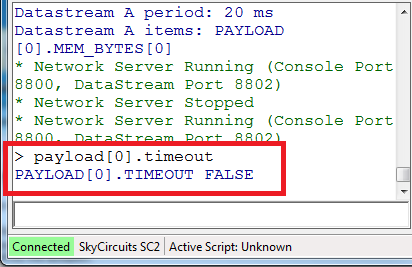
\includegraphics[width=0.5\textwidth]{testing_screenshots/timeout_false.png}
        \captionof{figure}{Timeout false on the customers ground station software shows that the payload is responding to transmit tokens correctly.}
        \label{fig:pl_comms_timeout_false}
\end{figure}


\begin{figure}[H]
        \centering
        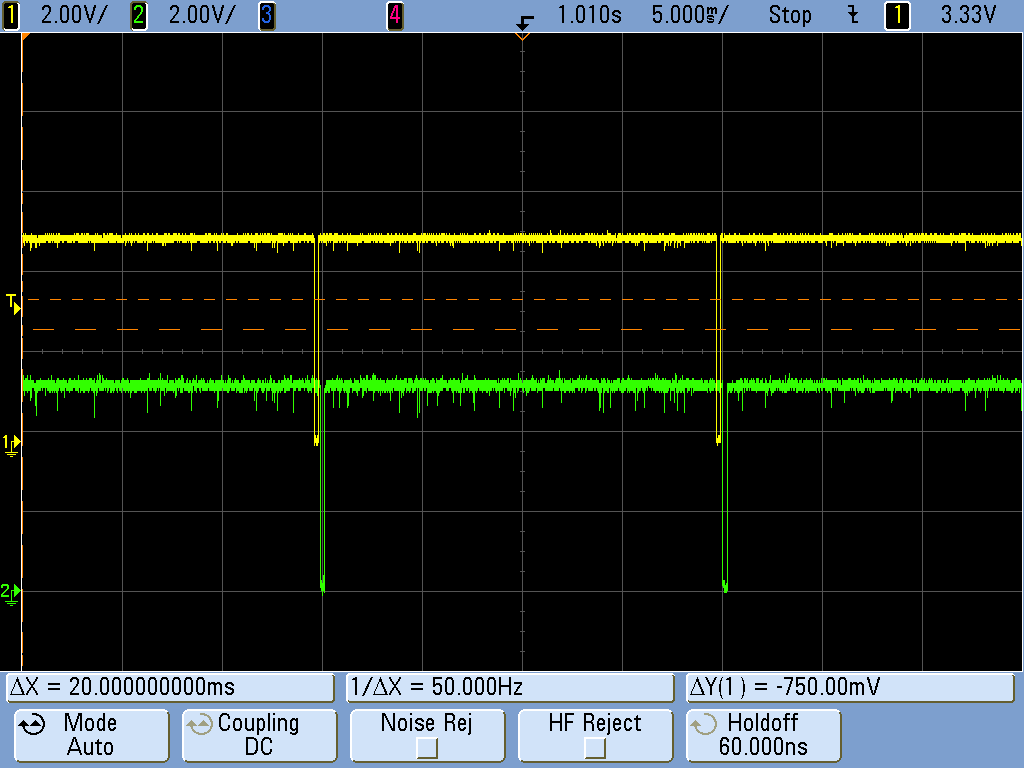
\includegraphics[width=0.75\textwidth]{testing_screenshots/transmit_tokens_succ.png}
        \captionof{figure}{Scope trace showing the autopilot sending the transmit token as the top trace (autopilot TX) and the payload responding as the bottom trace (autopilot RX.)}
        \label{fig:transmit_tokens_succ}
\end{figure}

\subsection{Test: Payload Setting Shared Memory on Autopilot}
\label{sec:test_pl_set_shared_mem}
This test simply attempts to validate the ability of the payload module to set shared memory on 
the autopilot. By setting the shared memory to one value on the ground station and then changing
it by setting it with the payload module we can verify the payload module has set the value correctly.

Figure \ref{fig:mem_bytes_test} shows the shared memory being set by the user
on the ground station software and then queried after the payload has set it - the memory
has changed to the value requested by the payload.

Milestone \ref{sec:ms_pl_shared_mem_set} is validated.

\begin{figure}[H]
        \centering
        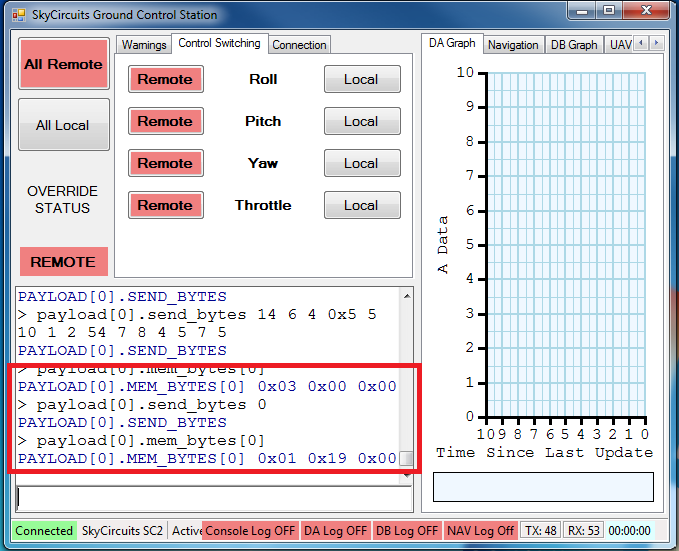
\includegraphics[width=1.0\textwidth]{testing_screenshots/mem_bytes_test.png}
        \captionof{figure}{mem\_bytes changes to the expected value after first query.}
        \label{fig:mem_bytes_test}
\end{figure}

\subsection{Test:  Payload Receiving Messages from Ground Station}
\label{sec:test_pl_receive_message}
This test attempts to validate the ability of the payload to receive and decode messages from the
autopilot. A message of length 1, content: 0x00 is sent using \verb+payload[0].send_bytes 0+ to
the payload through the ground station software. The debug connection is used to validate that the
correct message is received, shown in figure \ref{fig:send_bytes_test}. The test is successful
since the data is received by the payload as expected.

Milestone \ref{sec:ms_pl_rx_msg_gs} is validated.

\begin{figure}[H]
        \centering
        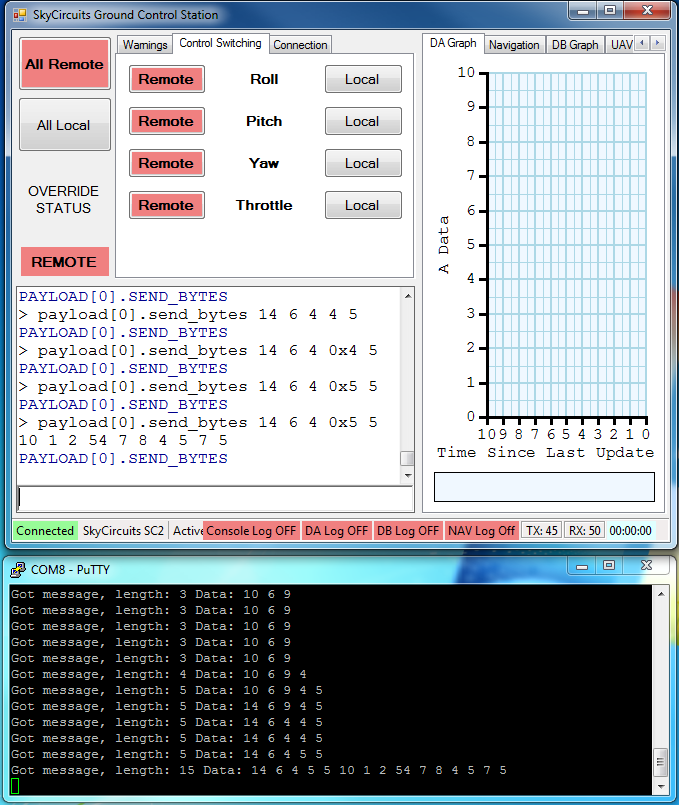
\includegraphics[width=1.0\textwidth]{testing_screenshots/send_bytes_test.png}
        \captionof{figure}{Payload (bottom) responding to send\_bytes command.}
        \label{fig:send_bytes_test}
\end{figure}


\subsection{Test: Image Sending to Ground Station via Autopilot Link}
\label{sec:test_pl_image_send}
Initially in order to test payload controller to ground station communications implementation
a PC console program was written to receive the incoming image data payload controller. By
inputting a \verb+payload[0].send_bytes 0+ command into the ground station software
the payload module triggers an image capture and the console application requests a download.

Figure \ref{fig:image_sending_test} shows the download of an image from the payload controller to
ground station via the autopilot link while figure \ref{fig:image_sending_test_example} shows an example
of an image downloaded. This test validates milestones \ref{sec:ms_pl_img_sending_gs} and \ref{sec:ms_pl_img_gs_trigger}.

\begin{figure}[H]
        \centering
        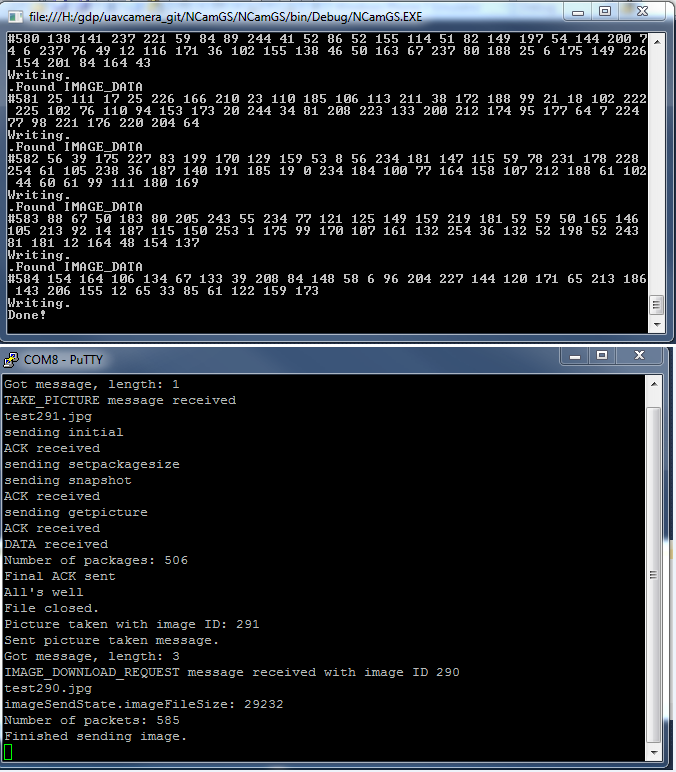
\includegraphics[width=1.00\textwidth]{testing_screenshots/image_sending_test.png}
        \captionof{figure}{Screenshot showing test of image capture and send via autopilot link. Top window is ground station console software recieving image and bottom console window is debug infomation from the payload controller.}
        \label{fig:image_sending_test}
\end{figure}

\begin{figure}[H]
        \centering
        \includegraphics[width=1.00\textwidth]{testing_screenshots/TEST30.jpg}
        \captionof{figure}{Example of image downloaded while testing payload to ground station image sending}
        \label{fig:image_sending_test_example}
\end{figure}
